

\let\negmedspace\undefined
\let\negthickspace\undefined
\documentclass[journal]{IEEEtran}
\usepackage[a5paper, margin=10mm, onecolumn]{geometry}
\usepackage{tfrupee} 

\setlength{\headheight}{1cm} 
\setlength{\headsep}{0mm}     

\usepackage{gvv-book}
\usepackage{gvv}
\usepackage{cite}
\usepackage{amsmath,amssymb,amsfonts,amsthm}
\usepackage{algorithmic}
\usepackage{graphicx}
\usepackage{textcomp}
\usepackage{xcolor}
\usepackage{txfonts}
\usepackage{listings}
\usepackage{enumitem}
\usepackage{mathtools}
\usepackage{gensymb}
\usepackage{caption}
\captionsetup{compatibility=false}
\usepackage{comment}
\usepackage[breaklinks=true]{hyperref}
\usepackage{tkz-euclide} 
\usepackage{listings}                                        
\def\inputGnumericTable{}                                 
\usepackage[latin1]{inputenc}                                
\usepackage{color}                                            
\usepackage{array}                                            
\usepackage{longtable}                                       
\usepackage{calc}                                             
\usepackage{multirow}                                         
\usepackage{hhline}                                           
\usepackage{ifthen}                                           
\usepackage{lscape}
\usepackage{amsthm}

\begin{document}

\bibliographystyle{IEEEtran}
\vspace{3cm}

\title{1.6.24}
\author{AI25BTECH11009 - Dasu Harshith Kumar}
{\let\newpage\relax\maketitle}

\renewcommand{\thefigure}{\theenumi}
\renewcommand{\thetable}{\theenumi}
\setlength{\intextsep}{10pt} 

\numberwithin{equation}{enumi}
\numberwithin{figure}{enumi}
\renewcommand{\thetable}{\theenumi}

\textbf{Question}: Find the values of \(k\) if the points  
A(2,3), B(4,k), C(6,-3) are collinear.\\\\

\textbf{Solution:}\\

We check collinearity using the vector method.  

\[
\vec{B}-\vec{A} = \myvec{4-2 \\ k-3} = \myvec{2 \\ k-3}
\]

\[
\vec{C}-\vec{A} = \myvec{6-2 \\ -3-3} = \myvec{4 \\ -6}
\]

Now form the matrix:  

\[
\vec{M} = \myvec{\vec{B}-\vec{A} & \vec{C}-\vec{A}}^T
= \myvec{2 & 4 \\ k-3 & -6}
\]

For collinearity, rank(\(M\)) = 1.  
That means the determinant of \(M\) must be zero:

\[
\det \myvec{2 & 4 \\ k-3 & -6} = -12 -4(k-3) = 0
\]

\[
-12 -4k + 12 = -4k = 0 \quad \Rightarrow \quad k = 0
\]

\[
\therefore \; A(2,3), B(4,0), C(6,-3) \; \text{are collinear for } k=0.
\]

\begin{figure}[htbp]
    \centering
    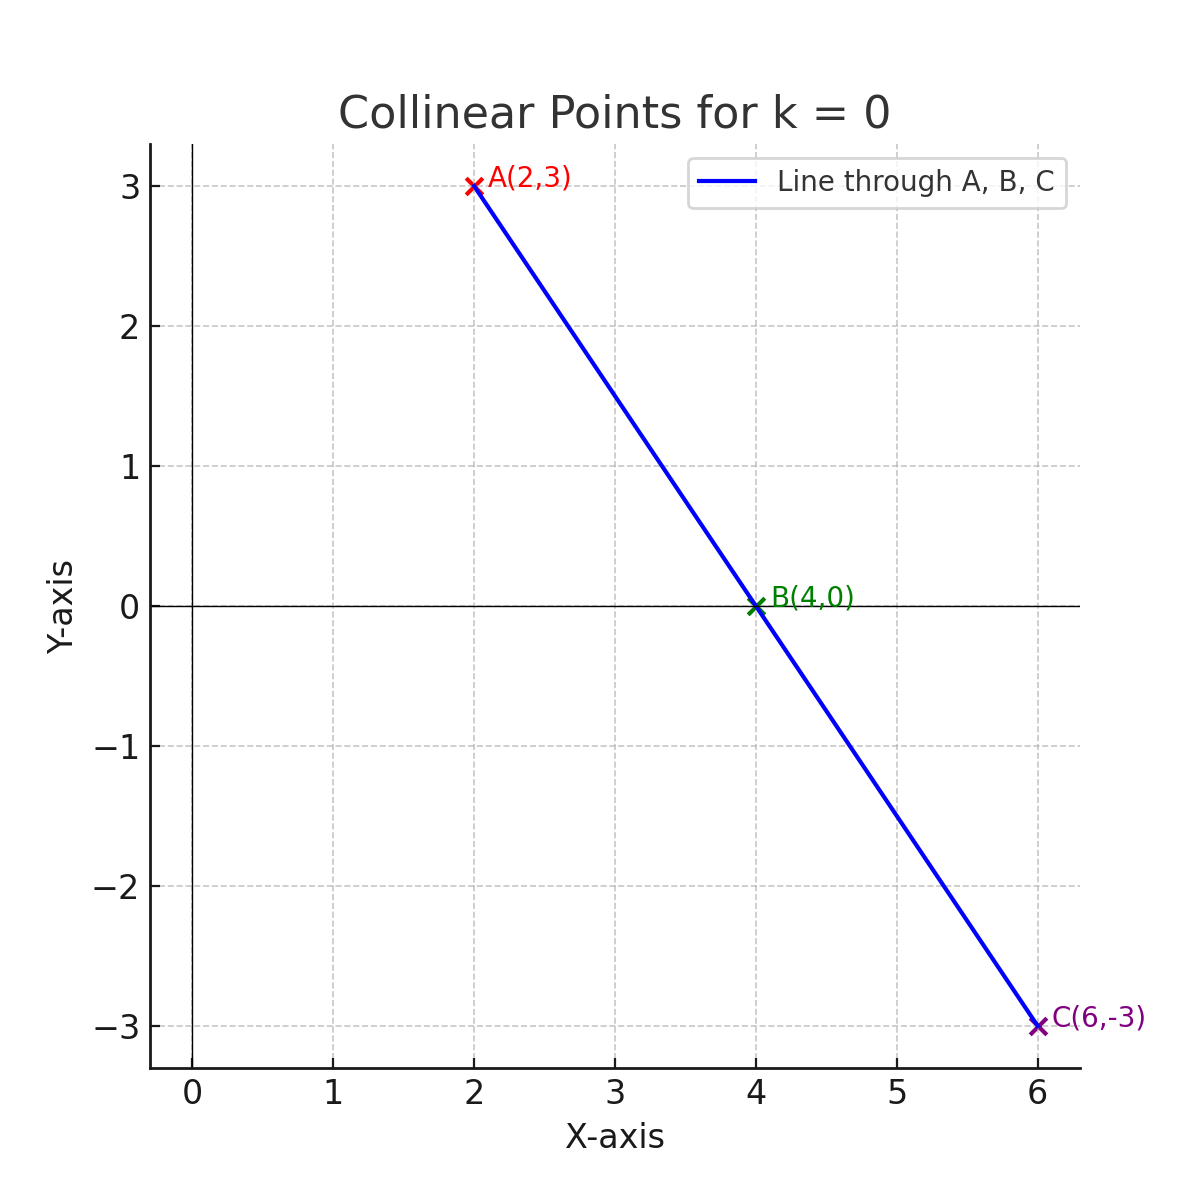
\includegraphics[width=0.8\linewidth]{figs/image.jpg}
    \caption{Graph showing collinear points A, B, C for \(k=0\)}
    \label{fig:fig1}
\end{figure}

\end{document}
